\documentclass[10pt,a4paper]{article}
\usepackage[T1]{fontenc}
\usepackage{lmodern}
\usepackage[utf8]{inputenc}
\usepackage[margin=20mm]{geometry}
\usepackage{graphicx,booktabs,array,xcolor,fancyhdr}
\usepackage[font=small,labelfont=bf,hypcap=false]{caption}
\usepackage[hidelinks]{hyperref}
\hypersetup{pdftitle={A Trusted Silver Layer for Great Britain Road Collision Analysis},pdfauthor={Faustine Caux and Jules Gombert},pdfsubject={DAT535 project report, University of Stavanger}}
\definecolor{accent}{RGB}{25,83,105}
\pagestyle{fancy}\fancyhf{}\fancyhead[L]{\small DAT535 --- STATS19 Data Pipeline}\fancyhead[R]{\small Group 16}\fancyfoot[C]{\thepage}
\setlength{\headheight}{14pt}
\setlength{\parindent}{0pt}\setlength{\parskip}{6pt}
\newcommand{\heading}[1]{\section*{\color{accent}#1}}
\newcommand{\subheading}[1]{\subsection*{#1}}
\newcommand{\code}[1]{\texttt{\detokenize{#1}}}
\begin{document}
\begin{center}
{\LARGE\bfseries A Trusted Silver Layer for Great Britain\\[4pt] Road Collision Analysis}\par
{\large Bronze--Silver--Gold batch processing with PySpark}\par
\textbf{Faustine Caux and Jules Gombert}\\[3pt]
University of Stavanger\\[3pt]
Group 16 \quad | \quad DAT535 \quad | \quad 11 November 2026
\end{center}
\heading{1. Problem, data and project scope}
The project transforms Department for Transport (DfT) STATS19 data into reusable, validated analytical tables. Its main engineering contribution is the Silver layer: retaining the correct record grains, interpreting official codes and checking relationships before publication. A focused Gold analysis demonstrates how those tables can answer the following question:

\begin{quote}\bfseries Which lighting, road-type and speed-limit profiles account for the largest numbers of fatal or serious reported collisions in Great Britain, 2021--2025?\end{quote}

The intended consumer is a road safety analyst choosing groups for closer local investigation. The analysis distinguishes absolute caseload, the proportion of collisions classified fatal or serious within a profile, and the profile's share of all severe collisions. These measures describe recorded collisions; traffic volumes and distance travelled are unavailable.

\begin{center}
\begin{tabular}{lrr}
\toprule Source table & Records & CSV size (decimal MB)\\\midrule
Collisions & 513,801 & 97.67\\
Vehicles & 937,265 & 103.74\\
Casualties & 652,821 & 53.69\\\bottomrule
\end{tabular}
\end{center}

The approximately 255 MB snapshot covers 2021--2025 and describes police-reported personal injury collisions in Great Britain. It excludes unreported events and does not represent every road accident. The official Excel data guide supplies category definitions. Original download dates were not recorded; validation timestamps must not be presented as acquisition dates. SHA-256 hashes identify the exact local input files, while mutable ``last five years'' URLs alone cannot reproduce a historical snapshot.

\subheading{Architecture and reproducibility}
Bronze preserves the three raw CSVs and reference guide. Silver publishes collision, vehicle and casualty Parquet tables plus a collision-level enriched table. Gold produces ten small summaries in Parquet and CSV, consumed by an executed notebook and generated figures. Scripts contain reusable transformations; notebooks serve interpretation and presentation.

The implementation uses Python 3.11, Spark 3.5.0 and Java 8 on the course VM. Separate development and production configuration files share the input snapshot but select different output directories. The repository contains source code, configuration, reference metadata and presentation evidence. Large raw inputs and generated layer directories are excluded from Git. Reproduction requires the externally retained CSVs whose hashes match the versioned baseline.

From the \code{project} directory, the main commands are:
\begin{quote}\small\ttfamily
bash scripts/run\_tests.sh\\
bash scripts/run\_project.sh --env dev\\
python scripts/render\_results.py --env dev
\end{quote}
The last command runs in the documented Python environment. Paths and Spark settings can be overridden without editing transformations.

\newpage
\heading{2. Bronze and Silver: preserving meaning and grain}
\subheading{Bronze validation and provenance}
Bronze acquisition is manual. The validator checks input presence, non-zero size, essential headers and duplicate column names, then records file sizes, SHA-256 hashes, column lists and change status. The reference guide is also hashed. Each attempt receives a distinct run directory and machine-readable report; the original CSVs remain unchanged. Checksums detect changed files, rather than duplicate records. Changed data still requires human review of schema, coverage and code definitions.

\subheading{A relational Silver model}
\begin{center}\small
\begin{tabular}{lp{49mm}p{67mm}}
\toprule Table & Grain & Key\\\midrule
Collisions & One reported collision & \code{collision_index}\\
Vehicles & One vehicle within a collision & \code{collision_index}, \code{vehicle_reference}\\
Casualties & One casualty within a collision & \code{collision_index}, \code{casualty_reference}\\\bottomrule
\end{tabular}\end{center}

A direct collision-level join of vehicles and casualties would multiply records: two vehicles and three casualties yield six joined rows. Instead, each child table is aggregated independently before joining its counts and attributes to collisions. The enriched table must retain exactly one row per collision. The original three tables remain available for other analytical questions, avoiding a flattened model tied to one report.

\begin{center}
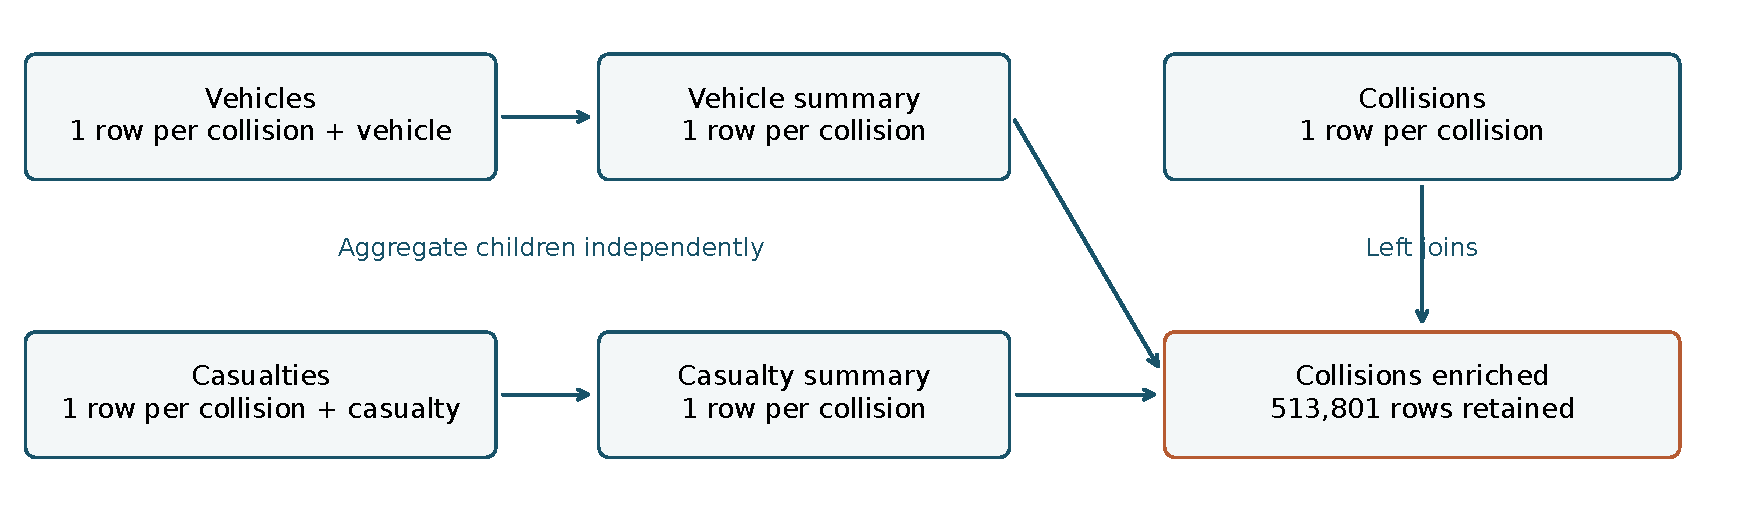
\includegraphics[width=\linewidth,height=45mm,keepaspectratio]{../figures/silver_model.pdf}
\captionof{figure}{Independent child aggregation preserves collision grain before enrichment.}
\end{center}

\subheading{Targeted transformations}
Numeric CSV types are inferred, with collision identifiers, reference strings and time explicitly preserved as text. This protects leading zeroes and avoids interpreting an \code{HH:mm} value as a timestamp. Dates are parsed into Spark dates; month, hour and weekend fields are derived. Conversion failures and inconsistencies against source year and weekday are counted.

Official labels are added for seven categorical fields: collision severity, casualty severity, weather, lighting, road surface, road type and vehicle type. The original codes remain available. Recognised unknown categories are distinguished from codes absent from the selected guide. Main severity codes remain distinct from enhanced severity categories; no severity adjustment is applied.

Age code $-1$ means ``Data missing or out of range''. Keeping it in a numerical average would bias the result; deleting the whole record would lose useful information. Silver therefore preserves source ages and adds nullable clean columns. Negative ages become null there, while unexpected negative codes trigger review. Zero is valid for casualties. For example, $-1,20,40$ becomes null, 20, 40: the recorded-age average is 30, with a denominator of two, and all three records remain.

Similarly, a clean speed-limit column retains the six recognised public-highway limits, in mph. Missing or unknown source values remain traceable in the original field and become a separate missing group in Gold. Missing coordinates are counted rather than used as a blanket reason for rejection.

\newpage
\heading{3. Quality evidence, tests and publication}
The reference development run is \code{20261110T150552746288Z}. Its Silver report passed all implemented gates. Input and output counts agree at every source grain:
\begin{center}
\begin{tabular}{lrrrr}
\toprule Table & Input & Output & Missing keys & Duplicate excess\\\midrule
Collisions & 513,801 & 513,801 & 0 & 0\\
Vehicles & 937,265 & 937,265 & 0 & 0\\
Casualties & 652,821 & 652,821 & 0 & 0\\\bottomrule
\end{tabular}\end{center}

There were no unmatched collision relationships, casualty-to-vehicle orphans, parent/child year mismatches, or discrepancies between observed child counts and source collision counters. There were no date/time conversion failures, calendar inconsistencies, unsupported speed values or unmapped codes in the seven decoded fields. All four Silver Parquet tables were reloaded and checked for row-count and data-type agreement.

The report also records limitations rather than hiding them: 142,240 driver ages and 14,106 casualty ages use the missing-age code; 53 longitudes and 53 latitudes are absent; three speed limits are coded missing. Recorded ages span 1--105 for drivers and 0--105 for casualties. These extrema are observations, not independent validation of each age. Coordinate range checks establish global plausibility, not geographic accuracy. No source records were removed.

\begin{center}
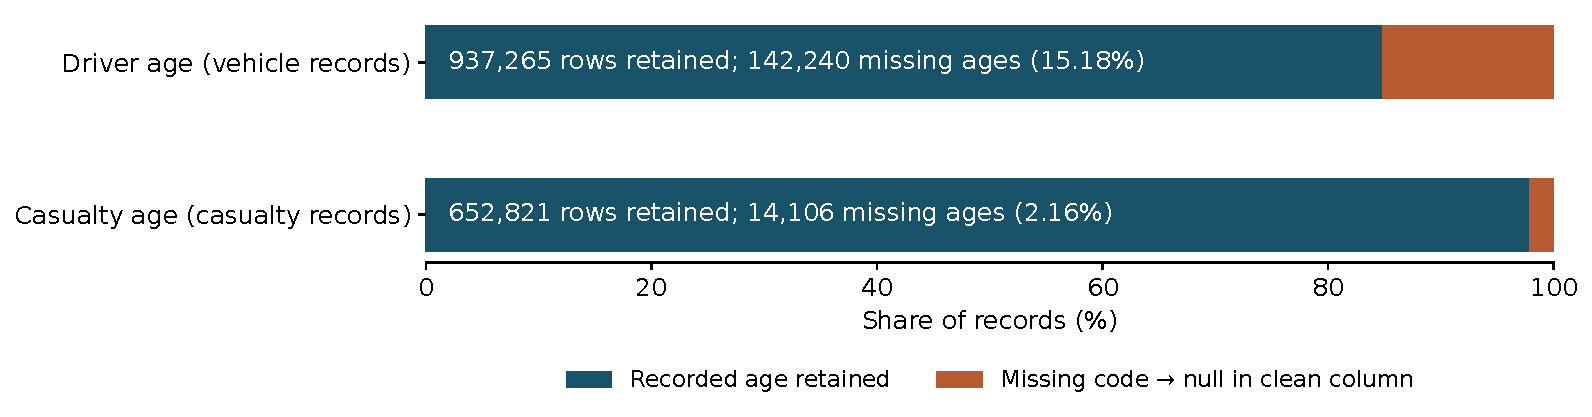
\includegraphics[width=\linewidth,height=43mm,keepaspectratio]{../figures/silver_age_quality.pdf}
\captionof{figure}{Missing-age information is made explicit without removing records. Source age null counts are zero; populated missing codes explain the clean-column nulls.}
\end{center}

\subheading{Complementary checks and failure behaviour}
Key checks enforce table grain. Foreign-key checks detect orphans. Comparing observed children with collision counters tests completeness relative to the parent's declarations. Checking enriched collision counts guards against join multiplication. These checks address different failure modes; none alone establishes complete data correctness.

Missing or duplicate keys and empty source tables cause failure. Relationship anomalies, unsupported categories and other implemented quality violations block Silver publication. A run requiring review does not proceed to Gold. Reports are written before successful pointers are replaced atomically, and failed outputs remain inspectable. A file lock prevents simultaneous full runs using the same operational directory.

Publication is atomic per pointer, not a transaction spanning every layer. Silver can advance before a later Gold failure. Consumers needing a consistent end-to-end snapshot should use the pipeline manifest and its run identifiers. Standalone stages should not run concurrently against shared outputs.

\newpage
\heading{4. Silver validation and execution evidence}
\subheading{Tests for the model and its quality gates}
The saved test evidence records \textbf{17 successful tests}. Small synthetic fixtures and temporary directories make the suite independent of the large CSVs. The versioned official guide is its only source-data dependency. Tests address record meaning, relational structure and failure behaviour:

\begin{center}\small
\begin{tabular}{p{40mm}p{112mm}}
\toprule Test area & Behaviour checked\\\midrule
Identifiers and grain & Leading zeroes and time text survive CSV loading; missing and duplicate keys are detected at the correct grain.\\
Codes and preparation & Guide-derived severity lists stay distinct; unknown codes are retained; clean ages exclude negative codes; invalid dates and unknown speeds are handled.\\
Enrichment & Two vehicles and three casualties produce one enriched collision with the expected child counts, rather than six joined rows.\\
Publication and lineage & Failed and review-required runs preserve successful pointers; Gold refuses unvalidated Silver; Bronze detects input changes.\\
End-to-end analysis & Totals reconcile; vehicle memberships are deduplicated; pooled and annual profiles use the correct reference populations.\\\bottomrule
\end{tabular}\end{center}

The failed-update integration test removes one vehicle from a previously valid fixture. Silver detects the inconsistency and requires review; Gold is skipped, and the previous Silver and Gold pointers remain unchanged. Expected failure messages in this test are successful detection, rather than a failing suite. This provides stronger evidence than checking only a valid example.

\subheading{Execution and performance choices}
The reference development run took 81.37 s: Bronze 0.95 s, Silver 59.49 s and Gold 19.48 s, plus orchestration overhead. A retained production manifest also reports a passed full run (74.00 s). Silver dominates the observed duration because it performs repeated audits, relationship checks and validated writes. These are observations from the VM, not service-level guarantees.

Transformations use built-in DataFrame operations; the monthly Gold summary uses Spark SQL. Source frames are cached for repeated audits, joins and writes, then unpersisted. Eight shuffle partitions are a small-VM starting point. Saved plans expose aggregations, scans, joins and shuffles. Silver avoids excessive year/month directory partitions at this volume; small Gold tables use one Parquet file each.

A separate experiment compares the same three-column yearly aggregation on CSV and Silver Parquet. An explicit CSV schema, no Spark cache and alternating format order make the comparison more interpretable. All query results match:
\begin{center}
\begin{tabular}{lrrrr}
\toprule Format & Trial 1 (s) & Trial 2 (s) & Trial 3 (s) & Median (s)\\\midrule
CSV & 6.0336 & 1.0380 & 0.7430 & 1.0380\\
Parquet & 1.4044 & 0.3758 & 0.2923 & 0.3758\\\bottomrule
\end{tabular}\end{center}
The Parquet plan shows a batched three-column scan; both formats use partial aggregation and a shuffle. Uncontrolled JVM warm-up, OS page cache and VM load prevent a general speedup claim. The benchmark references an earlier validated run on the same snapshot. A killed process during concurrent Spark activity motivated sequential runs with conservative memory settings on the 8 GB VM.

\newpage
\heading{5. Gold: a focused application of validated Silver}
Gold demonstrates the analytical value of Silver through 180 pooled profiles and 803 observed annual profile combinations. Monthly, hourly, weather, lighting, road-type, speed-limit, weekend and vehicle-type summaries complete the ten outputs. Exclusive summaries reconcile to Silver globally and, for annual profiles, within each year. Vehicle-type groups overlap and cannot be summed into an overall total.

\textbf{Daylight / single carriageway / 30 mph accounts for the largest severe caseload: 35,130 fatal or serious collisions, or 28.247\% of all severe collisions.} The five leading profiles contain 78,008 severe cases (62.725\%). Across the snapshot, 124,366 of 513,801 recorded collisions are fatal or serious (24.205\%).

\begin{center}
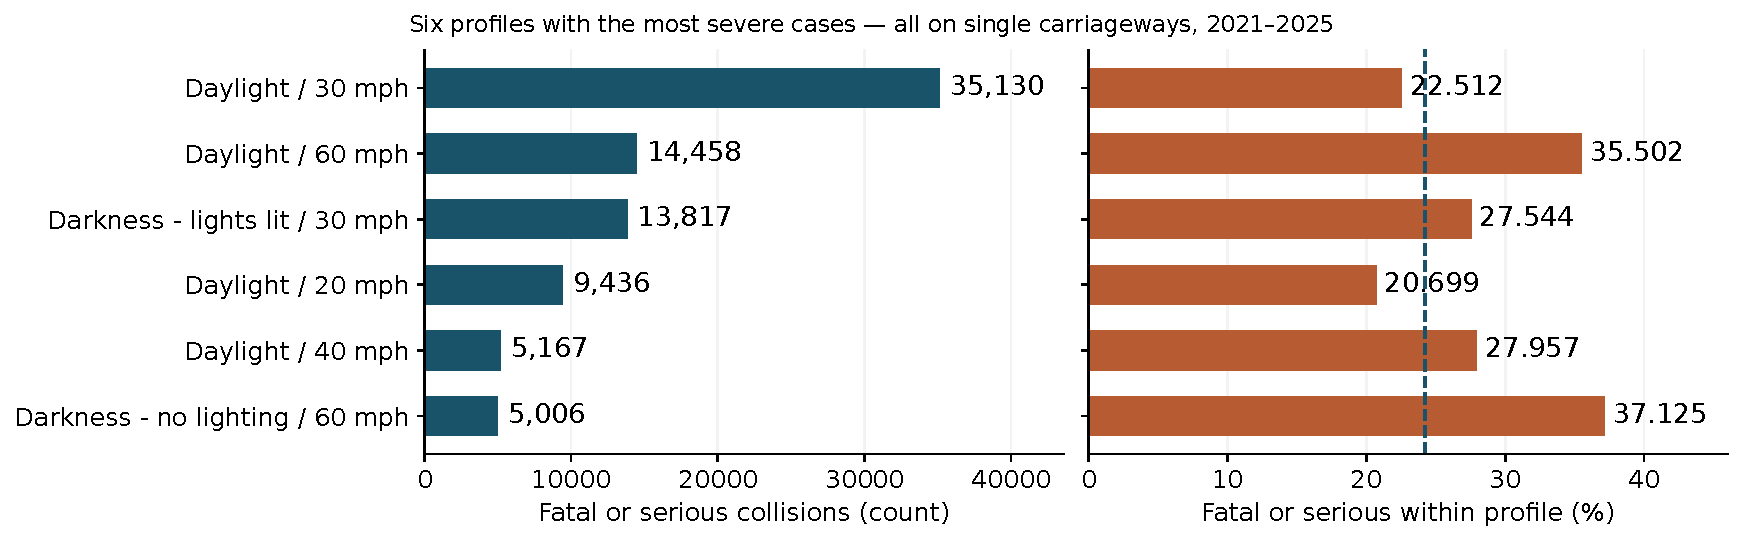
\includegraphics[width=\linewidth,height=67mm,keepaspectratio]{../figures/report_profiles.pdf}
\captionof{figure}{Absolute caseload and within-profile severity answer different questions. The dashed line is the overall severe proportion (24.205\%).}
\end{center}
The leading profile's within-profile severe proportion is 22.512\%, below the overall 24.205\%. Its share of all collisions is 30.371\%, compared with 28.247\% of severe cases: a gap of $-2.124$ percentage points. Its large caseload accompanies a large recorded collision population. Darkness without lighting / single carriageway / 60 mph has fewer severe cases (5,006), but a higher severe proportion (37.125\%). Its severe-case share exceeds its share of all collisions by 1.401 points. Neither comparison measures traffic exposure.

\begin{center}
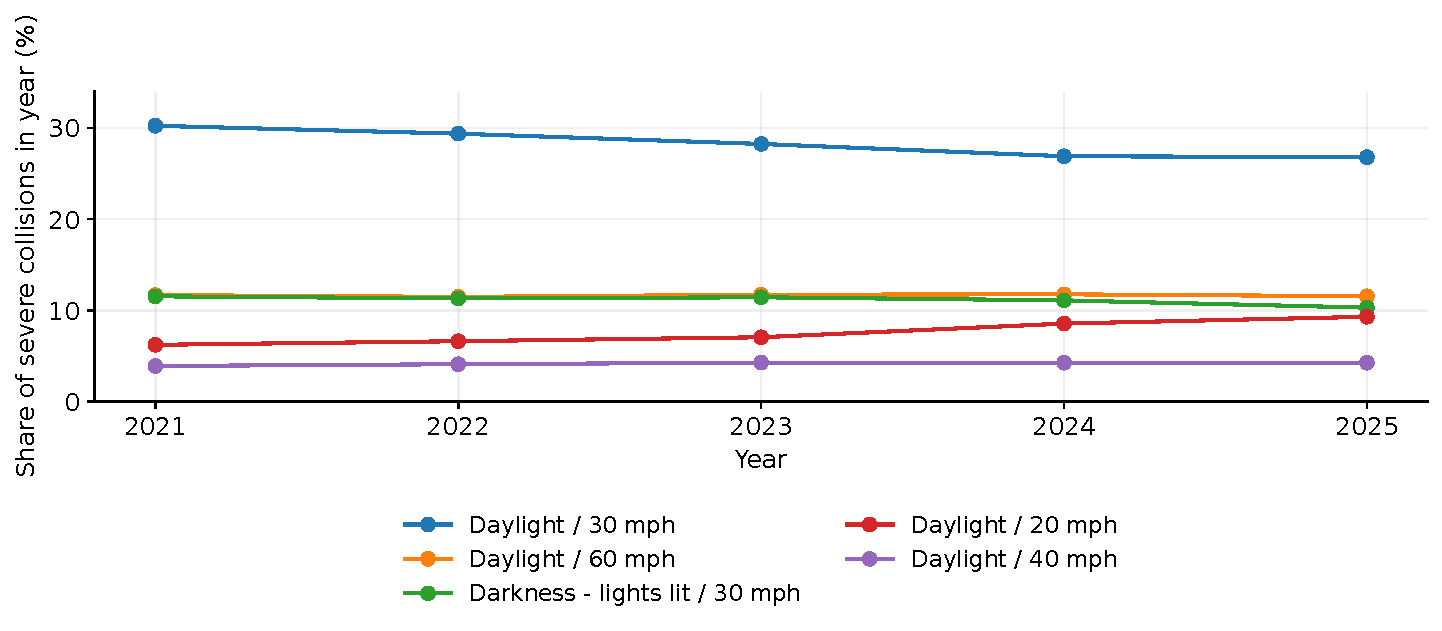
\includegraphics[width=\linewidth,height=60mm,keepaspectratio]{../figures/report_profile_years.pdf}
\captionof{figure}{Pooled leading profiles followed across years, using each year's severe-case total as the denominator.}
\end{center}
\textbf{The same five profiles retain ranks 1--5 in the same order every year from 2021 to 2025.} The leading profile has a negative severe-minus-all share gap in all five years; the unlit 60 mph comparison has a positive gap in all five. This is descriptive consistency within the observed period. Selection uses pooled data, and reporting changes remain relevant.

An analyst can use these groups to select local investigations, then obtain location, traffic-exposure and infrastructure information. The outputs cannot rank risk per kilometre or determine the effect of changing lighting or speed limits. Gold serves as a concrete consumer of Silver, rather than replacing its reusable model with a single ranking.

\newpage
\heading{6. Delivery, limitations and conclusion}
\subheading{CI/CD and operational delivery}
The project is merged into \code{main} at commit \code{e79206d}. The development workflow runs fixture tests on pushes to \code{dev}, same-repository pull requests targeting \code{dev}/\code{main}, and manual dispatch. Fork pull requests are excluded from the self-hosted test job. Test logs are retained as artifacts; legacy labs remain optional manual jobs.

The current production workflow runs on pushes to \code{main} or manual dispatch, executes tests followed by Bronze--Silver--Gold against the VM's external snapshot, then generates presentation artifacts. It uses a persistent production directory and the \code{main} environment. \textbf{Execution is triggered by a main-branch push or manual dispatch; no periodic schedule is currently enabled.} Environment approvals and required branch checks depend on GitHub settings and cannot be inferred from YAML or the merge. The retained production manifest identifies run \code{20261110T180208676518Z}. It establishes a passed execution in the production directory; the manifest alone does not identify the triggering GitHub event or establish environment approvals.

\subheading{Assessment artifacts and reproduction}
The repository entry point links this report, the executed notebook, analytical results and Silver quality evidence. The PDF and editable LaTeX source form the project report. A versioned copy of the reference Silver JSON report allows its key counts, schemas and checks to be inspected without the raw data or a running Spark installation. The report's new model, missing-age and profile figures can be regenerated from versioned evidence using \code{scripts/render_report_figures.py}.

Full reproduction additionally requires the original input snapshot and compatible Java/Spark/Python installations. Launchers accept external Bronze and output paths; the full pipeline manifest identifies a consistent run. Raw CSVs and generated layer datasets remain outside Git. Runtime directories are retained locally; long-term use requires a retention policy and monitoring of failed as well as successful attempts.

\subheading{Reflection and conclusion}
The strongest engineering choice is preserving relational grain while making publication depend on measured quality. Official-code interpretation prevents misleading age calculations; separate child aggregation prevents inflated collision counts. Keeping raw codes and nullable prepared fields improves traceability, although downstream users must still choose valid denominators.

This is a full-snapshot batch pipeline on one VM, not an incremental or multi-node platform. Priorities for expansion are explicit schema contracts, archived input versions, source-change review, retention policies and resource sizing based on measured workloads. The guide reader is tied to the selected workbook layout. Unknown acquisition dates, reporting bias, unadjusted severity and missing traffic exposure remain material limitations.

The central result is Silver: three reusable source-grain tables, collision-level enrichment and explicit evidence of structural consistency. Gold demonstrates their analytical use. The leading severe-case groups are consistent across the five observed years, while case volume and within-profile severity remain distinct. The result supports targeted investigation with clear boundaries on interpretation.

{\footnotesize\textbf{Sources and evidence.} DfT, \href{https://www.gov.uk/government/statistical-data-sets/road-safety-open-data}{Road safety open data}; DfT, \href{https://www.gov.uk/government/publications/guide-to-severity-adjustments-for-reported-road-casualty-statistics}{Severity adjustment guidance}. Repository evidence: analytical results and performance manifests in the reports directory, the executed analysis notebook and per-run quality reports. Contains public sector information licensed under the Open Government Licence v3.0.}
\end{document}
